\documentclass[times, 10pt]{thesisMDH}
\usepackage[ddmmyyyy]{datetime}
\usepackage[pdfborder={0 0 0},colorlinks=true,urlcolor=blue,citecolor=red,bookmarks=false]{hyperref}
\usepackage{float}
\usepackage{makecell}
% \usepackage{indentfirst}
\setlength\parindent{0pt}

\university{University of Science and Technology of Hanoi}
\department{Information and Communication Technology}

\subject{Distributed System}
\thesisTitle{Practical Work 2:\\RPC File Transfer}

\authorOne{Nguyen Phuong Thao}{BI9-212}
\authorTwo{Doan Tuyet Mai}{BI9-162}
\authorThree{Trinh Thao Phuong}{BI9-191}
\authorFour{Phung Kim Son}{BI9-202}
\authorFive{Pham Minh Long}{BI9-146}

\theDate{Hanoi, Feb 2021} 

\begin{document}
\titlePage

\newpage

\mainmatter

\section{Protocol design}
\begin{figure}[H]
    \centering
    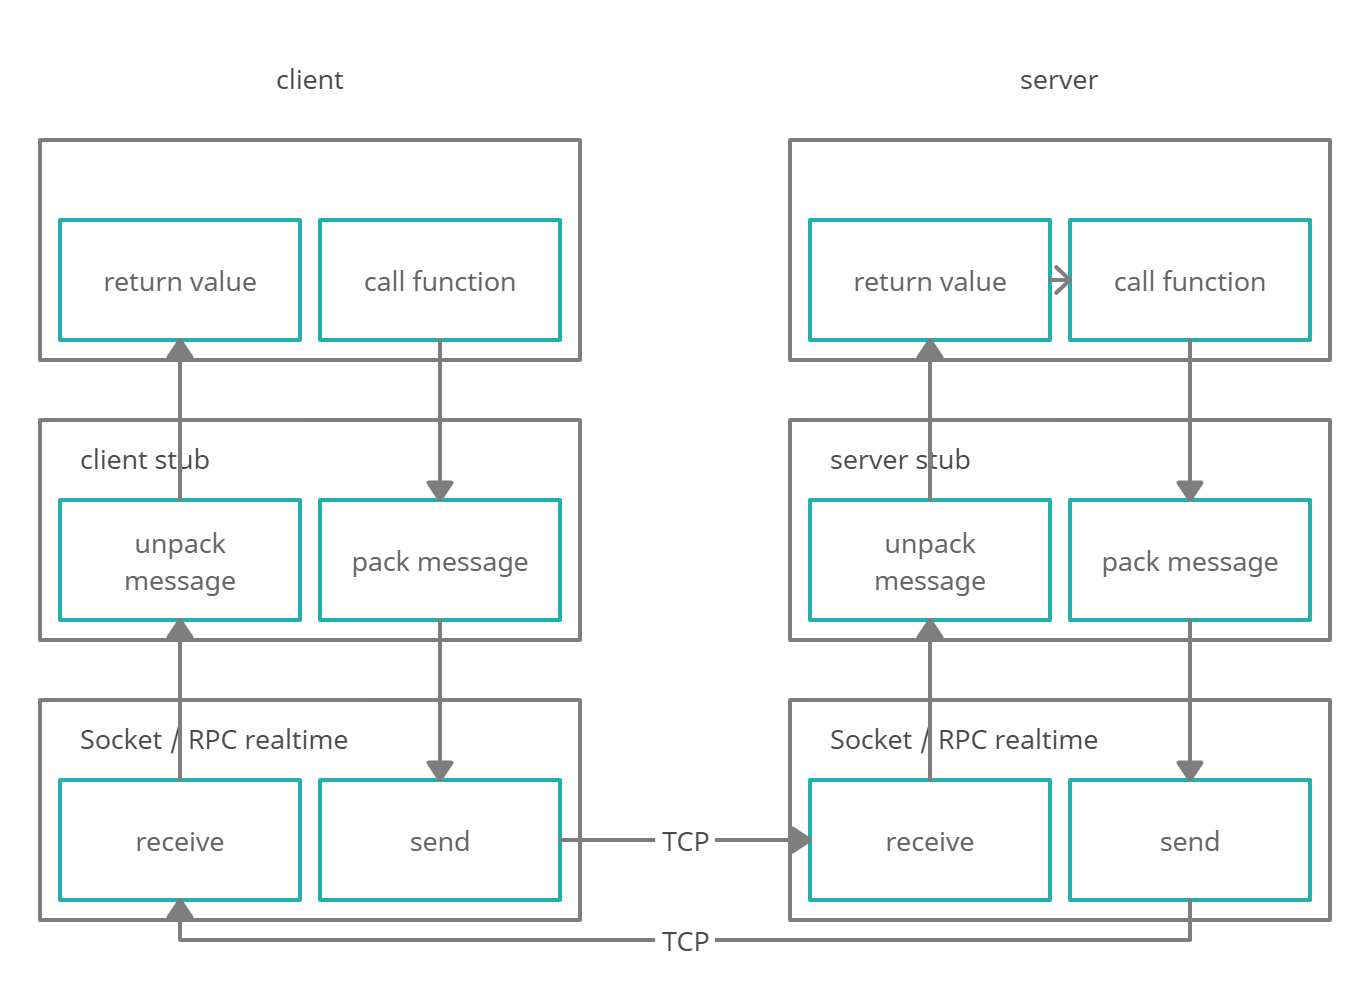
\includegraphics[width = 1\linewidth]{images/2-1.png}
    \caption{Protocol design}
\end{figure}
In RPC file transfer, the client makes a procedure call to send a
data packet to the server. When the packet is received, the server executes functions to performs what the client requests, packs reply into a message and makes the procedure call to returns messages to the client.

\section{System organization}
\begin{figure}[H]
    \centering
    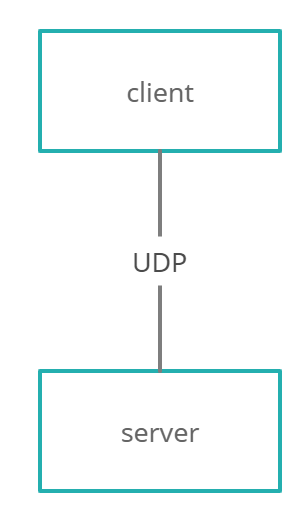
\includegraphics[width = 0.2\linewidth]{images/2-2.png}
    \caption{System organization}
\end{figure}
The server and client are connected together with the help of rpcgen through UDP. 

\section{File transfer implementation}
Full code implementation could be found \href{https://github.com/npthao1312/ds2021/tree/master/labwork2/code}{here}, in the \texttt{code} directory.\\[0.5em]
Client and server stubs were generated by \texttt{rpcgen}, using an input file \texttt{transfer.x} which contains interface definitions:
\begin{lstlisting}
#define SIZE 1024
typedef opaque filebytes[SIZE];

struct file {
	char name[SIZE];
	filebytes data;
	int nbytes;
};

program TRANSFER {
	version TRANSFER_1 {
		int TRANSF(file) = 1;
	} = 1;
} = 0x31230000;
\end{lstlisting}
Then, in the command line:
\begin{lstlisting}
$ rpcgen -a -C transfer.x
\end{lstlisting}
After that, output files to implement an RPC protocol will be generated.

\subsection{Client-side}
File transfer code for client-side was mainly implemented in \texttt{transfer\_client.c} file. Begin of the file is the include to the header file \texttt{transfer.h}\\[0.5em]
The client's RPC handle was created by \texttt{clnt\_create()}, which took the name of the remote host \texttt{host}, the program number \texttt{TRANSFER} and the program version \texttt{TRANSFER\_1} as parameters.
\begin{lstlisting}
CLIENT *clnt;
clnt = clnt_create (host, TRANSFER, TRANSFER_1, "udp");
if (clnt == NULL) {
	clnt_pcreateerror (host);
	exit (1);
}
\end{lstlisting}
Next, to talk about the file transfer, let's call the file that will be sent \texttt{sample}. This file will be first opened by \texttt{fopen()} to get the buffered input stream.
\begin{lstlisting}
fp = fopen(filetotransf, "rb");
if(fp == NULL) {
	printf("File not found.\n");
	exit(1);
}
\end{lstlisting}
If the file \texttt{sample} can't be opened, an alert will be printed.\\[0.5em]
After that, if the file size is larger than 1MB, it will be broken down into smaller parts, maximum size of each is 1MB, and then sent as arguments sequentially:
\begin{lstlisting}
while(1) {
	transf_1_arg.nbytes = fread(transf_1_arg.data, 1, SIZE, fp);
	result_1 = transf_1(&transf_1_arg, clnt);
	
	if (result_1 == (int *) NULL) {
		clnt_perror (clnt, "call failed");
	}

	if(transf_1_arg.nbytes < SIZE) {
		printf("Completed file transfer.\n");
		break;
	}
}
\end{lstlisting}

\subsection{Server-side}
File transfer code for server-side was mainly implemented in \texttt{transfer\_server.c} file. Begin of the file is the include to the header file \texttt{transfer.h}\\[0.5em]
The server's main function is  \texttt{transf\_1\_svc}. First, we will check if we are receiving the file and ready to open the file.   
\begin{lstlisting}
if (strcmp(opened_file, "") == 0 && fp == NULL) {
	printf("Receiving new file %s.\n", argp->name);

	strcpy(opened_file, argp->name);
	fp = fopen("received_sample", "ab+");
}
\end{lstlisting}
Then, we will begin to flush stream, and write data from the file in the stream. 
\begin{lstlisting}
if (strcmp(opened_file, argp->name) == 0) {
		fflush(stdout);

		fwrite(argp->data, 1, argp->nbytes, fp);

		if (argp->nbytes < SIZE) {
			printf("\nFinished receiving %s.\n", argp->name);
			total = 0;
			fclose(fp);
			fp = NULL;
			strcpy(opened_file, "");
		}
	}
\end{lstlisting}

\section{Contribution}
\begin{center}
    \begin{tabular}{|l|l|l|}
        \hline
        \textbf{Student} & \textbf{Student ID} & \textbf{Contribution}\\
        \hline
        Pham Minh Long & BI9-146 & Protocol design \\
        \hline
        Phung Kim Son & BI9-202 & System organization \\
        \hline
        Trinh Thao Phuong & BI9-191 & Draw figures, Brief explanation for protocol design \\
        \hline
        Doan Tuyet Mai & BI9-162 & \makecell[l]{Code for file transfer\\Explanation for the implementation of Client-side} \\
        \hline
        Nguyen Phuong Thao & BI9-212 & Explanation for the implementation of Server-side\\
        \hline
    \end{tabular}
\end{center}

\end{document}
